\documentclass[a4paper]{article}
\usepackage{amsmath}
\usepackage{stmaryrd}
\addtolength{\hoffset}{-2.25cm}
\addtolength{\textwidth}{4.5cm}
\addtolength{\voffset}{-3.25cm}
\addtolength{\textheight}{5cm}
\setlength{\parindent}{15pt}

\usepackage[unicode=true, colorlinks=false, hidelinks]{hyperref}
\usepackage[utf8]{inputenc}
\usepackage[english, russian]{babel}
\usepackage{mathtext}
\usepackage[T2A, TS1]{fontenc}
\usepackage{microtype} % Slightly tweak font spacing for aesthetics
\usepackage{amsthm, amssymb, amsmath, amsfonts, nccmath}
\usepackage{nicefrac}
\usepackage{epstopdf}
\usepackage[export]{adjustbox}
\usepackage{float} % Improved interface for floating objects
\usepackage{graphicx, multicol} % Enhanced support for graphics
\usepackage{pdfrender,xcolor}
\usepackage{breqn}
\usepackage{mathtools}
\usepackage{titling}
\usepackage{bm}
\usepackage{centernot}
\usepackage[cal=boondoxo,calscaled=.96]{mathalpha}
\usepackage{marvosym, wasysym} % More symbols
\usepackage{rotating} % Rotation tools
\usepackage{censor} % Facilities for controlling restricted text

\usepackage{fancyhdr}
\pagestyle{fancy}
\fancyhead{}\renewcommand{\headrulewidth}{0pt}
\fancyfoot[L]{}
\fancyhead{}
\fancyfoot{}
\fancyfoot[R]{\thepage}
\begin{document}
    \begin{titlepage}
   \begin{center}
       \vspace*{3cm}
       \large{САНКТ-ПЕТЕРБУРГСКИЙ ПОЛИТЕХНИЧЕСКИЙ УНИВЕРСИТЕТ}
       \vspace{0.4 cm}

       \large\textbf{Институт прикладной математики и механики}
       \vspace{0.4 cm}

       \large{Высшая школа прикладной математики и вычислительной физики}

       \vspace{3 cm}
       \normalsize\textbf{Отчет\\ по лабораторной работе №7\\ по дисциплине\\
«Математическая статистика»}
       \vfill
       \begin{flushright}
            \normalsize{Выполнил студент:\\
            Антонов Алексей\\
            группа: 3630102/80201}
            \vskip\medskipamount
            \normalsize{Проверил:

            к.ф.-м.н., доцент\\
            Баженов Александр Николаевич
            }
       \end{flushright}

       \vspace{0.8cm}


       \normalsize{Санкт-Петербург\\2021 г.}

   \end{center}
\end{titlepage}
    \tableofcontents
    \newpage
	\listoffigures
    \newpage
    \listoftables
    \newpage

\section {Постановка задачи}
\noindent Провести дисперсионный анализ с применением крритерия Фишера по данным регистраторов для одного сигнала.
Определить области однородности сигнала, переходные области, шум/ фон.
Длину сигнала взять равной 1024.

\section{Теория}
\noindent Необходимо вычислить следующие величины:
\begin{enumerate}
    \item Внутригрупповая дисперсия
    \begin{equation}
        s_{IntraGroup}^{2} = \frac{1}{k} \sum_{i=1}^{k} s_i^{2} = \frac{1}{k} \sum_{i=1}^{k} \frac{\sum_{j=1}^{n} (x_{ij}-X_{ср})^{2}}{k-1}
    \end{equation}
    где $X_{cp}$ -- среднее для части выборки; $k$ -- количество частей выборки; $n$ -- количество элементов в рассматриваемой части выборки.
    Внутригрупповая дисперсия является дисперсией совокупности и рассматривается как среднее значение выборочных дисперсий.
    \item Межгрупповая дисперсия
    \begin{equation}
            s_{InterGroup}^{2}  = k \frac{\sum_{i=1}^{k} (X_{i_{ср}}-X_{ср})^{2}}{k-1}
    \end{equation}
    где $X_{1_{cp}}, X_{2_{cp}}, \dots, X_{k_{cp}}$ -- среднее значение для под-выборок, $X_{cp}$ -- среднее значение этих мредних значений под-выборок.
    \item Значение критерия Фишера
    \begin{equation}
        F=\frac{s_{InterGroup}^{2}}{s_{IntraGroup}^{2}}
    \end{equation}
\end{enumerate}

\section{Ход работы}
\noindent На начальном этапе необходимо извлечь сигнал из исходных данных
(wave-ampl.txt).
Известно, что сигнал имеет длину 1024, поэтому необходимо
выбрать начальный индекс, кратный 1024.\\\\
\noindent Далее необходимо построить гистограмму, столбцы отвечают за
следующие подобласти:
\begin{itemize}
    \item фон (столбец с наименьшим значением)
    \item переходы (столбцы с малыми значениями)
    \item сигнал (второй по величине столбец после фона)
\end{itemize}
\noindent Перед определением областей однородности, необходимо устранить
явные выбросы.
Для этого был использован медианный фильтр (выброс =
среднее арифметическое его соседей).
По итогу получим сглаженный сигнал.
После устранения выбросов необходимо разделить сигнал на области
(сигнал, фон, переходные процессы). \\\\
\noindent Как только области получены, необходимо определить их тип.
Это
осуществляется с помощью применения критерия Фишера.
Если значение
критерия Фишера велико, это будут переходные процессы, если же значение
находится вблизи 1, то эти области однородны.

\section{Программная реализация}
\noindent Лабораторная работа выполнена на языке Python в среде PyCharm с использованием следующих библиотек:
 \begin{enumerate}
        \item math
        \item matplotlib
        \item numpy
 \end{enumerate}

\section{Результаты}
	\begin{figure}[H]
		\centering
		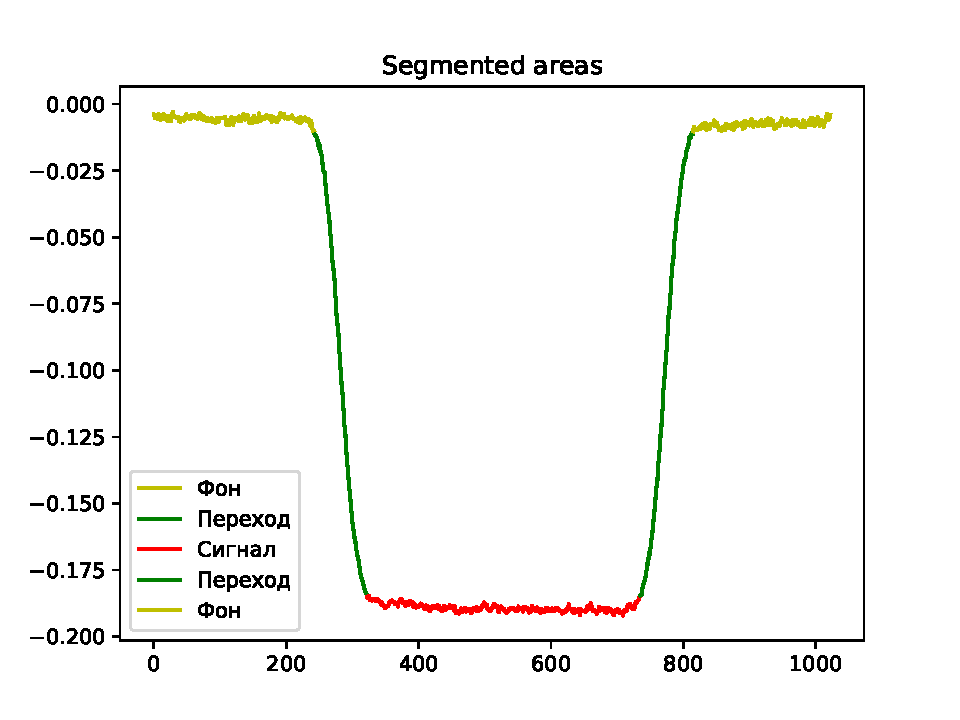
\includegraphics[width = 13cm, height = 8cm]{src/Segmented500}
		\caption{Изображение входного сигнала}
		\label{fig:signal}
	\end{figure}

		\begin{figure}[H]
		\centering
		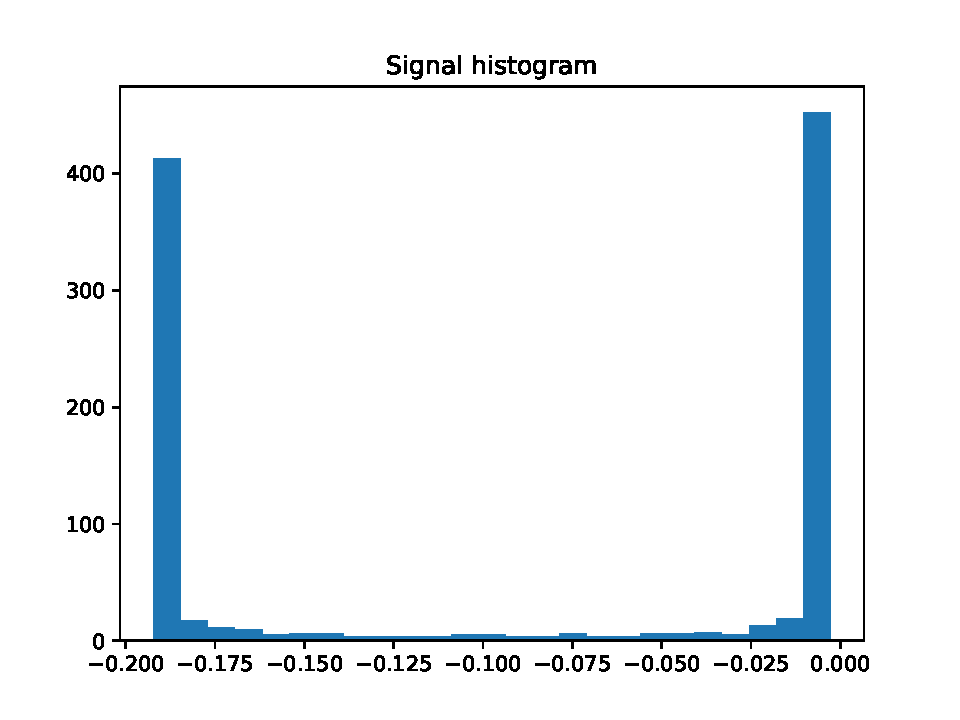
\includegraphics[width = 13cm, height = 8cm]{src/Signal500Hist}
		\caption{Гистограмма сигнала}
		\label{fig:signalHist}
	\end{figure}

	\begin{figure}[H]
		\centering
		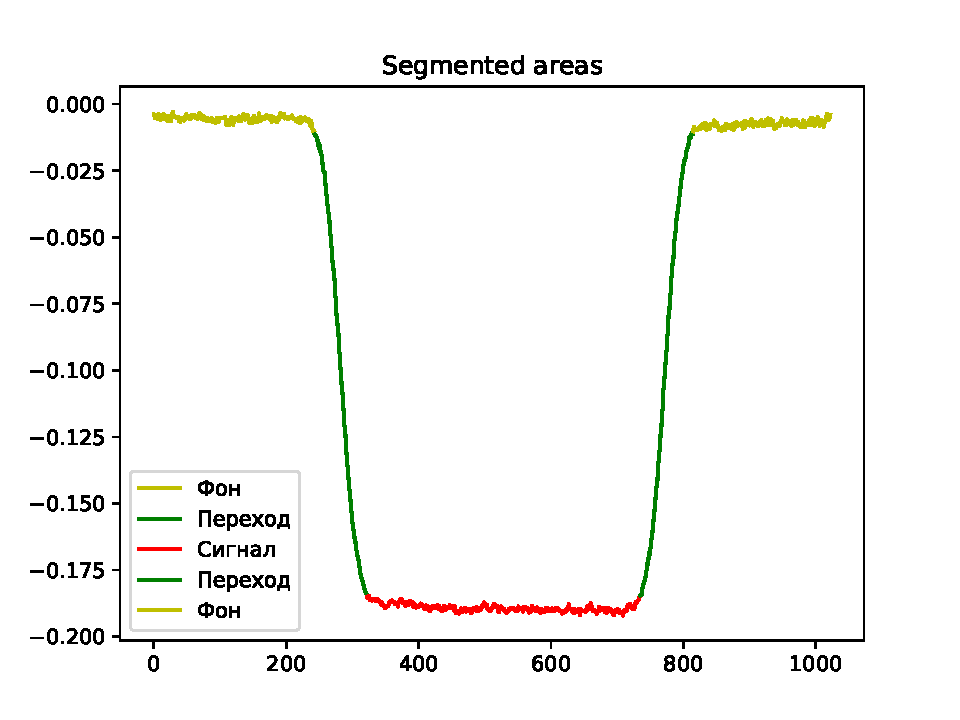
\includegraphics[width = 13cm, height = 8cm]{src/Segmented500}
		\caption{Разделение областей для данных сигнала}
		\label{fig:signalSegmented}
	\end{figure}
	\begin{table}[H]
    \centering
    \begin{tabular}{|c|c|c|c|}
    	\hline
        Промежуток&Тип&Количество разбиений&Критерий Фишера\\ \hline
1&Фон&9&1.3668\\ \hline
2&Переход&4&19.3068\\ \hline
3&Сигнал&7&1.0187\\ \hline
4&Переход&4&19.5921\\ \hline
5&Фон&4&0.1866\\ \hline

    \end{tabular}
    \caption{Характеристики выделенных областей}
    \label{tab:FisherTab}
\end{table}
\section{Обсуждение}
\subsection{Проверка гипотезы о законе распределения генеральной совокупности. Метод хи-квадрат}

\noindent Заключаем, что гипотеза $H_{0}$ о нормальном законе распределения $N(x,\hat{\mu}, \hat{\sigma})$ на уровне значимости $\alpha = 0.05$ согласуется с выборкой для нормального распределения $N(x, 0, 1)$.
\\
Также видно, что для выборок сгенерированных по равномерному закону и закону Лапласа гипотеза $H_{0}$ оказалась принята.

\section{Приложение}
    С кодом работы и отчета можно ознакомиться по ссылке:\;\url{https://github.com/sqrtyyy/MathStat/tree/master/lab_8}

\end{document}
